% !TEX root = ../thesis.tex

In this section we introduce the Belief Propagation (BP) algorithm for tree-structured MRF which, we show, is an iterative algorithm that can recover functions -- the beliefs -- proportional to the exact node marginals by passing ``messages'' through the graph \citep{pearl88,wainwright08}. We also show how this algorithm can be related to the two-filter formula for smoothing on a HMM discussed in chapter \ref{chap:BIS}.

We then introduce the Loopy Belief Propagation (LBP), an extension of the BP algorithm on graphs with cycles. This algorithm does not lead to functions proportional to the exact node marginals but recovers proxies for it which work well in practice \citep{yedidia02,sudderth03}.

In line with the rest of this document we concern ourselves with the case where the state-spaces associated with the graph nodes are continuous

\subsection{Belief Propagation on a tree}

%\dred{Should revisit this, explain a touch more how this comes to life, also see if the extension to cliques as opposed to single node is trivial or not. It may or may not be relevant, think!}
%\dred{Go back to the original equations and suggest how one can compute the integrals in a tree from the leaf nodes to a root node blah blah blah BP updates}

%\subsubsection{Tree graphs}

The problem of computing singleton marginals on a tree is relatively easy since the recursive structure of the problem can be exploited. Let $s$ denote a node of interest so that we are targeting the marginal $p(x_{s})$. 
The full joint on the tree can then be written relative to that node:
\eqa{	p(x) &\propto& \psi_s(x_s) \prod_{t\in\partial s} \psi_{ts}(x_t,x_s)\pac{\psi_t(x_t)\phi_{\partial t\backslash s}(x_t,x_{\partial t\backslash s})},	\label{eq:factorisation-tree}}
where the $\phi_{\partial t\backslash s}$ are given recursively by
%
\eqa{	
	\phi_{\partial t\backslash s}(x_t,x_{\partial t\backslash s}) 
		&=& \prod_{r\in\partial t\backslash s} \psi_{rt}(x_r,x_t)\pac{\psi_r(x_r)\phi_{\partial r\backslash t}(x_r,x_{\partial r\backslash t})},	\nn}
%
and $\phi_\emptyset \equiv 1$ (for a leaf node). 
This decomposition is illustrated at figure \ref{BP for tree 1}.
%%
\begin{figure}[!h]
\center
\begin{tikzpicture}[-,minimum size=1.1cm,scale=.1,node distance=2cm, thick]
	\node[circle,draw](A) {$s$};
	\node[](Al)[left = 2cm of A] {$\psi_s$};
	\node[circle,draw](B) [below left = 1.2cm and 0.3cm of A] {$t$};
	\node[](Bl)[left = 0.91cm of B] {$\psi_t$};
	\node[](ABl)[above = 0cm of Bl, xshift=0.05cm]{$\psi_{ts}$};
	\node[](C) 	[below right = 1.2cm and 0.3cm of A] {};
	\node[](Ba)	[below left = 1cm and -0.1cm of B] {};
	\node[](Bb)	[below right = 1cm and -0.1cm of B] {};
	\node[ellipse, minimum height=1.5cm,minimum width=3cm,draw=none,fill=DarkBlue!10](Bc)[below = 0.5cm of B] {$\phi_{\partial t\backslash s}$};
	\node[](D)[right = 2.05cm of ABl] {};
	\path
	(A) edge [line width=0.2pt,draw=DarkBlue](Al)
	(B) edge [line width=0.2pt,draw=DarkBlue](Bl)
	(ABl) edge [line width=0.2pt,draw=DarkBlue] (D)
	(A) edge  (B)
	(A) edge [dashed] (C)
	(B) edge [dashed] (Ba)
	(B) edge [dashed] (Bb)
	;
\end{tikzpicture}
\caption{\label{BP for tree 1} Illustration of the elements of the factorisation \eqref{eq:factorisation-tree}: the node potential $\psi_{s}$ of the node of interest, the potential corresponding to the edge connecting it to one of its neighbour $t$: $\psi_{st}$, the potential at that node, and the product of all subsequent potentials attached to that node $\phi_{\partial t\backslash s}$.}
\end{figure}

Using this recursive factorisation, and integrating out all variables apart from $x_{s}$, the marginal of interest can be written as
\eqa{		p_{s}(x_{s}) &\propto& \psi_{s}(x_{s})\prod_{t\in\partial s} \int \psi_{ts}(x_{t},x_{s}) \pac{\psi_{t}(x_{t})\underbrace{\int \phi_{\partial t\backslash s}(x_{t},x_{\partial t\backslash s}) \dx_{\partial t\backslash s}}_{=:\kappa(x_{t})}}\dx_{t}.\nn	}
Exploiting the recursive structure of $\phi_{\partial t\backslash s}$, we can expand the $\kappa$ term:
\eqa{	\kappa(x_{t}) &=& \prod_{r\in \partial t\backslash s} \int \psi_{rt}(x_r,x_t)\pac{\psi_r(x_r)\int\phi_{\partial r\backslash t}(x_r,x_{\partial r\backslash t})\mathrm{d}x_{\partial r\backslash t}}\mathrm{d}x_{r}.\nn}
Consequently, we can write
\eqa{		\hspace*{-.5cm}p_{s}(x_{s}) &\propto& \psi_{s}(x_{s})\prod_{t\in\partial s}m_{t s}(x_{s})	\nn}
where the \emph{messages} $m_{ts}$ are defined as
\eqa{	m_{t s}(x_s) &:=& \int \psi_{ts}(x_t,x_s)M_{ts}(x_t)\,\mathrm{d}x_t,	}
and the \emph{pre-messages} $M_{ts}$ as
\eqa{	M_{ts}(x_t) &:=& \psi_t(x_t) \prod_{r\in\partial t\backslash s}m_{r t}(x_t),	}
with, for a leaf node $\alpha$, $M_{\alpha  s} \equiv \psi_\alpha$. This is the BP algorithm which can be described more compactly as starting with the pre-messages on the leaf-nodes of the tree and propagating using the following equations:
\eqa{		\syst{	M_{st}(x_{s}) &=& \psi_{s}(x_{s}) \prod_{r\in\partial s\backslash t} m_{rs}(x_{s}) \\
				m_{ts}(x_{s}) &=& \int\psi_{st}(x_{s},x_{t})M_{ts}(x_{t})\dx_{t}\\
				B_{s}(x_{s}) &=& m_{ts}(x_{s})M_{st}(x_{s})	}.	\label{eq structure bp}}
The $B_{s}(x_{s})$ are known as the \emph{beliefs} and are proportional to the true marginals as we showed with the development above. \check{aug17}

\subsection{Belief propagation on a chain}
A particular case of interest is the chain graph which is associated with Hidden Markov Models introduced at section \ref{intro:exMRF} and studied in more details at chapter \ref{chap:BIS}. On the leaf node, we have a prior $\pi_{0}(x_{1})$ and an observation with likelihood $p(y_{1}\st x_{1})$. Therefore, we have $M_{12}(x_{1})=\pi_{0}(x_{1})p(y_{1}\st x_{1})\propto p(x_{1}\st y_{1})$. Correspondingly, the message $m_{12}$ is given by
\eqa{
	m_{12}(x_{2}) &\propto& \int p(x_{2}\st x_{1}) p(x_{1}\st y_{1}) \dx_{1} \spe p(x_{2}\st y_{1}).\nn
}
\subsubsection{Forward messages}
Let us assume that $m_{t-1, t} \propto p(x_{t}\st y_{1:t-1})$ (prediction density). Then, the next pre-message is:\footnote{Using $p(x_{t}\st y_{1:t})= p(x_{t},y_{1:t-1},y_{t})/p(y_{1:t})\propto p(y_{t}\st x_{t})p(x_{t}\st y_{1:t-1})$.}
\eqa{
	M_{t,t+1}(x_{t}) &\propto& p(y_{t}\st x_{t})p(x_{t}\st y_{1:t-1}) \esp\propto\esp p(x_{t}\st y_{1:t}).
}
Consequently, the next message can be computed thereby verifying our earlier assumption:
%
\eqa{		m_{t, t+1}(x_{t+1}) &\propto& \int p(x_{t+1}\st x_{t})p(x_{t}\st y_{1:t})\dx_{t} \spe p(x_{t+1}\st y_{1:t}).	}
%
\subsubsection{Backward messages}
In a similar way, we now start with a leaf node with no prior, i.e.: $M_{T,T-1}(x_{T})=p(y_{T}\st x_{T})$ and hence
%
\eqa{
	m_{T,T-1}(x_{T-1}) 
		&=& \int p(x_{T}\st x_{T-1})p(y_{T}\st x_{T})\dx_{T} \esp\propto\esp p(y_{T}\st x_{T-1})\nn.		
}
%
Let us assume that $M_{t+1, t}(x_{t+1}) \propto p(y_{t+1:T}\st x_{t+1})$. Noting that we can write the joint distribution on $(x_{t},x_{t+1}, y_{t+1:T})$ in two equivalent ways:
%
\eqa{		
	p(x_{t},x_{t+1},y_{t+1:T}) 
		&=& p(x_{t+1}\st y_{t+1:T},x_{t})p(y_{t+1:T}\st x_{t})p(x_{t})\nn\\
		&=& p(y_{t+1:T}\st x_{t+1})p(x_{t+1}\st x_{t})p(x_{t})	\nn
}
%
we have that $p(x_{t+1}\st y_{t+1},x_{t})p(y_{t+1:T}\st x_{t}) = p(y_{t+1:T}\st x_{t+1})p(x_{t+1}\st x_{t})$. Using the update equation for a message and our earlier assumption about the form of the pre-messages, we have
%
\eqa{
	m_{t+1, t}(x_{t}) 
		&\propto&\int p(x_{t+1}\st x_{t})p(y_{t+1:T}\st x_{t+1})\dx_{t+1} \nn\\
		&\propto& \int p(x_{t+1}\st y_{t+1:T},x_{t})p(y_{t+1:T}\st x_{t})\dx_{t+1} \nn\\		
		&\propto& p(y_{t+1:T}\st x_{t}).	}
%
We can then confirm our earlier assumption since
\eqa{		M_{t, t-1} &\propto& p(y_{t}\st x_{t})p(y_{t+1:T}\st x_{t})\esp\propto\esp p(y_{t:T}\st x_{t}),}
which shows that the backward messages on a HMM are  $p(y_{t+1:T}\st x_{t})$.
Summarising, on a HMM, we have that the forward messages ($t$ to $t+1$) correspond to the predictive densities and the forward pre-messages correspond to the filtering densities whilst the backward pre-messages correspond to the backward information filters discussed in chapter \ref{chap:BIS}.

%%%%%%%%%%%%
\subsubsection{Beliefs}
Now that the messages have been defined explicitly, we can write the beliefs as
%
\eqa{
	B_{t}(x_{t}) 
		&=& m_{t-1,t}(x_{t}) M_{t,t-1}(x_{t})\nn\\
		&\propto& p(x_{t}\st y_{1:t-1})p(y_{t:T}\st x_{t}) 
}
%
which is the two filter formula for the smoothing distribution $p(x_{t}\st y_{1:T})$ which we had introduced at point \ref{point:TFS}.

%%%%%%%%%%%%%%%%%%%%%%%%%%%
\subsection{\label{point:LBP}Loopy Belief Propagation}

In the presence of cycles in the graph (\emph{loopy graph}), there is not a unique way to go through all nodes. 
Propagating messages through different orderings of the nodes can therefore lead to inconsistent messages (see \ref{fig:lbp-inconsistent} for an illustration).
 
\begin{figure}[!h]
\center
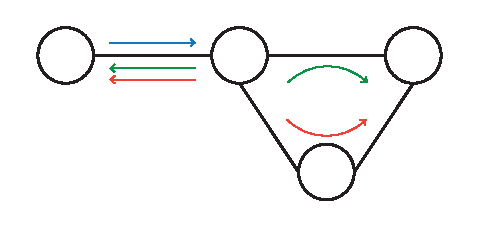
\includegraphics[width=.7\textwidth]{figures/lbp/loopy1}
\caption{\label{fig:lbp-inconsistent}A simple graph with a loop. Starting from the leaf node (blue arrow), the message can be propagated in the loop following a clock-wise ordering (green arrow) or a anti-clockwise ordering (orange arrow). The two backward messages coming back to the leaf node do not necessarily match. (This graph is best seen in colours.)}
\end{figure}

A common workaround is to perform the BP algorithm multiple times on different spanning trees of the graphs corresponding to different ordering of the nodes and hope that the iterations converge to a fixed point. This is know as the \emph{loopy belief propagation} (LBP) algorithm \citep{pearl88, yedidia02}:
%
\eqa{		\syst{	M_{st}^{n}(x_{s}) &=& \psi_{s}(x_{s}) \prod_{r\in\partial s\backslash t} m^{n-1}_{r s}(x_{s}) \\
				m^{n}_{ts}(x_{s}) &=& \int \psi_{ts}(x_{t},x_{s})M^{n}_{ts}(x_{t})\dx_{t}\\
				B^{n}_{s}(x_{s}) &=& m^{n}_{ts}(x_{s})M^{n}_{s t}(x_{s})	}.	\label{eq structure lbp}
				}
%
The initial messages are usually chosen among a class of simple distributions (e.g., the Normal distribution) potentially incorporating prior knowledge about the steady state messages. 
Provided the algorithm converges to a fixed point, the beliefs cannot be guaranteed to be proportional to the true marginals unlike the tree case. However, the beliefs can provide good approximations to the marginals which makes the LBP a popular method for approximate Bayesian inference on MRFs \citep{sudderth03}. The fixed points of the LBP have been shown to correspond to extrema of the Bethe free energy \citep{yedidia02} and there exist conditions under which the LBP algorithm provably converges \citep{heskes04,ihler05}.

Note that while it is known that the LBP algorithm can lead to good proxy to the marginals, the updates may still be intractable. Indeed, the computation of messages requires an integral which may be hard (or expensive) to compute accurately (e.g., if the dimension of the random variable on a node is high).\check{aug17}







